\documentclass{article}
\usepackage[utf8]{inputenc}
\usepackage{url}
\usepackage{graphicx}
\usepackage{float}
\usepackage[export]{adjustbox}
\graphicspath{ {images/} }

% code listing config
\usepackage{listings}
\lstset{
    basicstyle=\footnotesize\ttfamily,
    breaklines=true,
    tabsize=4,
    keepspaces=true,
    columns=flexible,
    % backgroundcolor=\color[gray]{0.9},
    frame=single
}

\title{Embedded Systems Laboratory \\
        MSP430 microcontroller}
    \author{
  Snoeijs, Jan\\
    \texttt{jan.snoeijs@epfl.ch}
  \and
  Spieler, Michael\\
  \texttt{michael.spieler@epfl.ch}
}
\date{17 October 2017}

\begin{document}

\maketitle

\section{Global configurations}

The clock configuration is the same for the whole program. In the main function we define the values in the \verb'BCSCTL' registers as well as the \verb'DCOCTL' so that the main clock, and sub-main clock are sourced by the digitally controlled oscillator (DCO) configured at a frequency of 1 MHz with no further frequency division. The Auxillary Clock (ACLK) runs on the LFXT1 internal low frequency oscillator at 32768 Hz. The watchdog timer is disabled and global interrupts are enabled through the GIE flag. The GPIO P1.3 pin is set to output low to provide a GND connection for the potentiometer.

\section{Timer A configuration for interrupt}

We used timer A1 to generate interrupts every 50 ms to trigger the analog to digital conversion. We configured the Timer A1 in counting-up mode to a value stored in \verb'TCCR0', and enabled the interrupts by setting the TAIE flag in the \verb'TA1CTL' register. The timer is clocked by the \verb'SMCLK' source at 1MHz. Inside the \verb'TimerA1_ISR' interrupt routine the ADC conversion is triggered by setting the ADC10SC bit in the ADC control register. This bit is reset to 0 by hardware. The resulting 50ms period was measured with the logic analyzer as shown in Figure \ref{fig:adc}.

\begin{figure}[H]
    \centering
    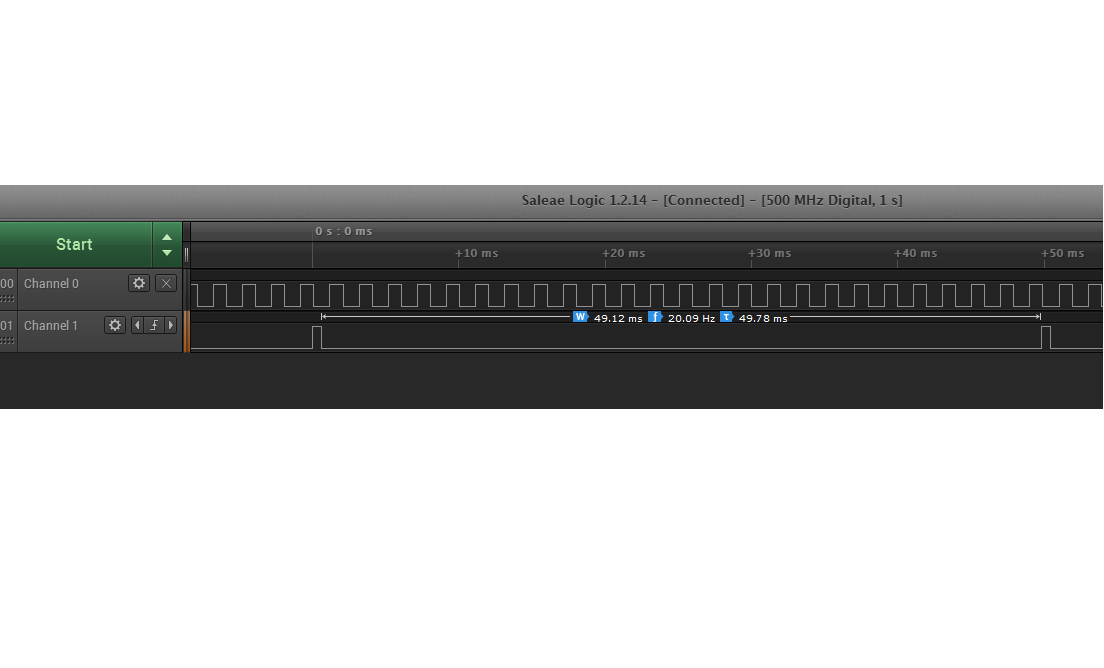
\includegraphics[width=\textwidth]{images/Capture2}
    \caption{Channel 0: PWM output, Channel 1: rising edge = TimerA1 interrupt, falling edge = ADC10 interrupt. The ADC is triggered every 50ms}
    \label{fig:adc}
\end{figure}

\section{ADC10 analog-to-digital converter configuration}
We configure the ADC10 for single channel conversion using channel A1 from pin P1.1. The ADC runs on the internal ADC10OSC clock with a prescaler of 8. The sample-and-hold time is set to 64x ADC10CLKs.
After configuration the ADC10 is enabled using the \verb'ENC' bit in \verb'ADC10CTL0' and then conversion is triggered by setting the ADC10SC bit, as described above.
The GPIO analogue input function is selected through the \verb'ADC10AE0' for P1.1.
After a conversion the \verb'ADC10_ISR' interrupt routine is called where we read the result from \verb'ADC10MEM' and and adjust the PWM duty cycle.
Finally the \verb'ADC10IFG' interrupt flag is cleared before returning from the ISR.

\section{PWM signal generation}

To generate a PWM signal we use the timer A0 which is counting up to a fixed value (TACCR0).
Its clocking is done the same way as for the interrupt-timer A1, that is SMCLK at 1 MHz source, without divider. The timer is configured in Up mode, which counts to \verb'TCCR0' register.
Thus the PWM period is controlled by the \verb'TCCR0' value in microseconds.
The capture compare unit 1 is configured for OUTMODE7 which is Set/Reset. Thus the duty time is controlled by the \verb'TCCR1' register value in microseconds.
The \verb'PWM_set_duty()' function to change the duty cycle, which is called form the ADC interrupt. The initial duty time is set to 1 ms.
Figure \ref{fig:pwm} shows an example PWM output for 0.8ms duty time and a period of 2ms.

\begin{figure}[H]
    \centering
    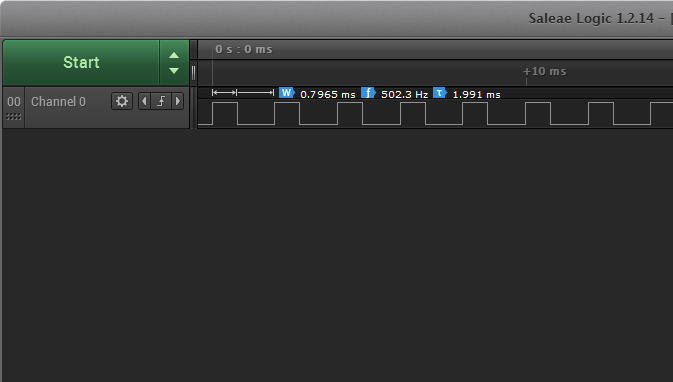
\includegraphics[scale=0.5]{images/Capture1}
    \caption{Example of output PWM signal}
    \label{fig:pwm}
\end{figure}

\section{Direct ADC triggering from hardware timer}
The AD conversion can be triggered from a timer compare output directly.
This solution removes the need for an interrupt service routine and thus removing the software and execution overhead.
To do this \verb'SHSx' bits must be set to 0b10 to select \verb'Timer0_A.OUT0' as the sample-and-hold source.
Since the ADC triggers on a rising edge the timer must be run at double frequency if OUT0 toggles on a compare match.
Because of lack of time this solution was not implemented.


\section{Source Code}

\begin{lstlisting}[
    language=C++,
    numbers=left,
    caption=main.c,
    label=lab1_main_c
]
#include <msp430.h>
#include <stdint.h>

void PWM_set_duty(uint16_t duty_time_us)
{
    TACCR1 = duty_time_us;
}

// setup Timer_A for 2ms period
void PWM_init(uint16_t duty_time_us)
{
    // GPIO P1.6 CCR1 output
    P1DIR |= BIT6;
    P1SEL |= BIT6;
    P1SEL2 &= ~BIT6;

    /* TimerA0 PWM configuration:
     * input clock SMCLK = 1MHz
     * reload: TACCR0 = 2000 - 1 => 500Hz or 2ms period
     * Up Mode
     * OUTMOD: Reset/Set
     */
    TA0CTL = TASSEL_2 | ID_0 | MC_1;
    TA0CCTL0 = 0;
    TA0CCR0 = 2000 - 1;
    TA0CCTL1 = CM_0 | OUTMOD_7;

    PWM_set_duty(duty_time_us);
}

void ADC_TimerA1_init(uint16_t period_us)
{
    /* TimerA1 periodic interrupt configuration:
     * input clock SMCLK = 1MHz
     * reload: TACCR0 = period_us - 1
     * Up Mode
     */
    TA1CTL = TASSEL_2 | ID_0 | MC_1 | TACLR;
    TA1CCTL1 = CM_0 | CCIS_0 | OUTMOD_0;
    TA1CCR0 = period_us;

    // enable timer interrupt
    TA1CTL |= TAIE;
}

#pragma vector=TIMER1_A1_VECTOR
__interrupt void TimerA1_ISR(void)
{
    TA1CTL &= (~TAIFG); // Clear TAIFG flag in TA0CTL register
    ADC10CTL0 |= ADC10SC;
}

/* Configure ADC input for P1.1 */
void ADC_init(void)
{
    /* ADC configuration:
     * single conversion
     * channel A1 (pin P1.1)
     * 64x sample-and-hold time
     * Conversion trigger via ADC10SC bit
     * ADC10OSC clock source about 5MHz
     */
    ADC10CTL0 = ADC10SHT_3 | ADC10SR | ADC10ON | ADC10IE | SREF_0;
    ADC10CTL1 = INCH_1 | SHS_0 | ADC10DIV_7 | ADC10SSEL_0 | CONSEQ_0;
    ADC10DTC1 = 0;

    ADC10CTL0 |= ENC;

    // P1.1 input
    P1DIR &= ~BIT1;
    ADC10AE0 |= BIT1;
}

uint16_t adc_val = 0;

#pragma vector=ADC10_VECTOR
__interrupt void ADC10_ISR(void)
{
    // Read conversion result
    adc_val = ADC10MEM;

    PWM_set_duty(800 + (uint32_t)400 * adc_val / 1023);

    // Clear ADC10IFG interrupt flag
    ADC10CTL0 &= ~ADC10IFG;
}

int main(void)
{
    // Stop watchdog timer
    WDTCTL = WDTPW | WDTHOLD;

    /* Clock configuration:
     * MCLK: 1MHz
     * SMCLK: 1MHz
     * ACLK: 32768Hz LFXT1 internal oscillator
     */
    DCOCTL = CALDCO_1MHZ;
    BCSCTL1 = CALBC1_1MHZ | XT2OFF | DIVA_0;
    BCSCTL2 = SELM_3 | DIVM_0 | DIVS_0;
    BCSCTL3 = XT2S_0 | LFXT1S_0 | XCAP_1;

    // P1.3 output low
    P1DIR |= BIT3;
    P1OUT &= ~BIT3;

    // setup PWM, 1ms duty time
    PWM_init(1000);

    ADC_init();
    ADC_TimerA1_init(50000); // trigger ADC every 50ms

    // Enable global Interrupt
    __bis_SR_register(GIE);

    while (1) {
        ;
    }
}
\end{lstlisting}

\end{document}
